\documentclass[11pt,aspectratio=169]{beamer}
\usepackage[utf8]{inputenc}
\usepackage[T1]{fontenc}
\usepackage[italian]{babel}
\usepackage{lmodern}
\usepackage{xcolor}
\usepackage{booktabs}
\usepackage{array}
\usepackage{colortbl}
\usepackage{graphicx}
\usepackage{tcolorbox}
\tcbuselibrary{skins}

\definecolor{accent}{HTML}{2B6E64}
\definecolor{accentsoft}{HTML}{E2EFEC}
\definecolor{warncol}{HTML}{A8500A}
\definecolor{warnsoft}{HTML}{FBEDE0}
\definecolor{goodcol}{HTML}{2F7D4F}
\definecolor{badcol}{HTML}{B0362F}
\definecolor{inksoft}{HTML}{4B5652}
\definecolor{inkfaint}{HTML}{7C8884}
\definecolor{bgcol}{HTML}{F4F6F5}

\newcommand{\good}[1]{\textcolor{goodcol}{\textbf{#1}}}
\newcommand{\warncell}[1]{\textcolor{warncol}{\textbf{#1}}}
\newcommand{\badcell}[1]{\textcolor{badcol}{\textbf{#1}}}
\newcommand{\dashcell}{\textcolor{inkfaint}{---}}

\usetheme{Madrid}
\usecolortheme{default}
\setbeamercolor{structure}{fg=accent}
\setbeamercolor{title}{fg=white,bg=accent}
\setbeamercolor{frametitle}{fg=white,bg=accent}
\setbeamercolor{background canvas}{bg=bgcol}
\setbeamercolor{block title}{fg=white,bg=accent}
\setbeamercolor{block body}{fg=black,bg=accentsoft}
\setbeamertemplate{navigation symbols}{}
\setbeamertemplate{footline}[frame number]

\title{Duplicate-Task Gaps in BPI12}
\subtitle{Dal dataset simulato alla causa radice: i limiti di Split Miner}
\author{Daniele Gelmini}
\date{\today}

\begin{document}

\begin{frame}
\titlepage
\end{frame}

\begin{frame}{In sintesi}
\begin{block}{}
Un modello predittivo allenato su dati \textbf{interamente simulati} dava previsioni quasi identiche indipendentemente dalla raccomandazione testata.
\end{block}
\vspace{0.5em}
\begin{itemize}
\item La causa finale non era il simulatore: era la \textbf{rete di Petri} minata da Split Miner
\item Split Miner: un'etichetta $\to$ una sola posizione nella rete (per costruzione)
\item Soluzione: \textbf{rinominare le attivit\`a nel log} prima della discovery
\item Risultato: eventi/traccia quasi identico al reale (\good{24.33} contro 24.55)
\end{itemize}
\end{frame}

\begin{frame}{Il problema originale}
\begin{columns}[T]
\column{0.55\textwidth}
\begin{itemize}
\item Training set interamente simulato per BPI12 (3737 tracce, come il reale)
\item Modello predittivo allenato su questi dati $\to$ previsioni \textbf{piatte}, quasi identiche per ogni rank di raccomandazione
\item Prima ipotesi: routing a \textbf{probabilit\`a fisse}, indipendente dalla storia del caso
\end{itemize}
\column{0.45\textwidth}
\begin{tcolorbox}[colback=warnsoft,colframe=warncol,title=Sintomo]
Nel pannello ``modello su dati simulati'', i punti dei diversi rank si sovrappongono quasi tutti
\end{tcolorbox}
\end{columns}
\end{frame}

\begin{frame}{Primo miglioramento: alberi decisionali}
\begin{center}
\begin{tabular}{lcc}
\toprule
\textbf{Metrica} & \textbf{Prob. fisse} & \textbf{Alberi (depth=2)} \\
\midrule
\% esito positivo (reale 48.3\%) & \warncell{30.2\%} & \good{48.7\%} \\
Eventi/traccia (reale 24.3) & 21.4 & \badcell{44.4} \\
\bottomrule
\end{tabular}
\end{center}
\vspace{1em}
\begin{itemize}
\item Instradamento condizionato sulla storia del caso $\to$ distribuzione dell'esito quasi perfetta
\item Ma: alcune attivit\`a di rework si ripetono troppo (ciclo ``gestione offerta'')
\end{itemize}
\end{frame}

\begin{frame}{Tre bug corretti nel simulatore}
\begin{enumerate}
\item \textbf{Tupla malformata} nella serializzazione JSON
\item \textbf{Alberi di routing senza regolarizzazione} $\to$ split su rumore (\texttt{AMOUNT\_REQ})
\item \textbf{Caso degenere}: \texttt{None} sempre convertito in peso \textbf{1}, anche quando la vera costante era \textbf{0}
\end{enumerate}
\vspace{1em}
\begin{center}
\begin{tabular}{lccc}
\toprule
& \textbf{Reale} & \textbf{Prima} & \textbf{Dopo} \\
\midrule
Eventi/traccia & 24.29 & \warncell{43--44} & \good{22.20} \\
\texttt{A\_CANCELLED}/traccia & 0.350 & ripete 5--7$\times$ & \badcell{0.000} \\
\bottomrule
\end{tabular}
\end{center}
\end{frame}

\begin{frame}{Split Miner: un'etichetta, un task}
\begin{tcolorbox}[colback=white,colframe=accent,boxrule=0.4pt,left=8pt]
\small\emph{``\ldots N is the non-empty set of nodes\textsuperscript{4}, for which exists \textbf{a bijective function l : N $\to$ L}\ldots''}\\
{\scriptsize\textsuperscript{4}``Each node of the graph represents a task.''}\\
\textcolor{inkfaint}{Augusto, Conforti, Dumas, La Rosa, Polyvyanyy --- ``Split Miner'', Definizione 3 (DFG)}
\end{tcolorbox}
\vspace{1em}
\begin{itemize}
\item Ogni etichetta $\to$ \textbf{esattamente un} task nella rete, sempre
\item Non discusso come limite nel paper: assunzione implicita
\item \texttt{A\_CANCELLED} nella rete: un solo predecessore ammesso (\texttt{W\_Nabellen offertes})
\item Nel log reale: 46.8\% arriva da \texttt{O\_CANCELLED} --- percorso assente
\end{itemize}
\begin{alertblock}{Verifica esatta}
\texttt{A\_CANCELLED} sincronizzato \textbf{0 volte su 181.979} righe; il cancello osservato \textbf{21.621 volte, mai scelto}
\end{alertblock}
\end{frame}

\begin{frame}{La regola generale: quando Split Miner tiene un arco}
Per ogni coppia di attivit\`a $(a,b)$ con traffico in \textbf{entrambe} le direzioni, Split Miner (Definizione 5 del paper, ``Pruned DFG'') decide con una sola formula:
\[
r = \frac{|freq(a{\to}b) - freq(b{\to}a)|}{freq(a{\to}b)+freq(b{\to}a)}
\]
\begin{columns}[T]
\column{0.5\textwidth}
\begin{tcolorbox}[colback=accentsoft,colframe=accent,title=Caso normale: $r \geq \varepsilon$]
Le due direzioni sono sbilanciate a sufficienza $\to$ \textbf{non} concorrenti. Si tiene solo l'arco \textbf{pi\`u frequente}; il pi\`u debole viene scartato.\\
\small\`E cos\`i per la stragrande maggioranza delle coppie nel log.
\end{tcolorbox}
\column{0.5\textwidth}
\begin{tcolorbox}[colback=warnsoft,colframe=warncol,title=Caso concorrenza: $r < \varepsilon$]
Le due direzioni sono troppo bilanciate $\to$ classificate \textbf{concorrenti} (``possono avvenire in qualsiasi ordine''). Si scartano \textbf{entrambi} gli archi, indipendentemente da quanto siano frequenti.
\end{tcolorbox}
\end{columns}
\vspace{0.6em}
{\small Quindi normalmente sopravvive sempre una direzione --- non \`e la regola, \`e l'eccezione a fare danno.}
\end{frame}

\begin{frame}{Il nostro caso: rientra nell'eccezione}
\begin{itemize}
\item \texttt{O\_CANCELLED $\to$ A\_CANCELLED}: \textbf{767} occorrenze --- l'arco pi\`u frequente in assoluto verso A\_CANCELLED (pi\`u di quello sopravvissuto, 732)
\item \texttt{A\_CANCELLED $\to$ O\_CANCELLED} (direzione opposta): \textbf{864} occorrenze
\end{itemize}
\[
r = \frac{|767-864|}{767+864} = \mathbf{0.059}
\]
\begin{itemize}
\item Con qualunque $\varepsilon$ ragionevole (paper: 0.1), $0.059 < \varepsilon$ $\to$ scatta il caso ``concorrenza'', \textbf{non} il caso normale
\item Risultato: l'arco pi\`u frequente in assoluto viene scartato insieme al pi\`u debole --- non perch\'e raro, ma perch\'e il traffico nelle due direzioni \`e quasi identico
\end{itemize}
\end{frame}

\begin{frame}{Ma allora perch\'e sembra sopravvivere un verso?}
Nella rete: dopo \texttt{A\_CANCELLED} l'unico passo possibile \`e \texttt{O\_CANCELLED} --- sembra che l'arco \texttt{A\_CANCELLED$\to$O\_CANCELLED} sia sopravvissuto. \textbf{Non \`e cos\`i}, verificato sulla rete:
\begin{center}
\small
\begin{tabular}{ll}
\toprule
\textbf{Alimenta \texttt{ent\_xor\_16}} (uscita A\_CANCELLED) & \textbf{Da dove} \\
\midrule
\texttt{A\_CANCELLED} & stesso bivio \\
transizione invisibile (scollegata da A\_CANCELLED) & stesso bivio \\
\bottomrule
\end{tabular}\\[4pt]
Unico consumatore: \texttt{O\_CANCELLED}
\end{center}
\begin{alertblock}{Il punto}
\texttt{ent\_xor\_16} \`e un posto di \textbf{join}: due rami alternativi confluiscono l\`i, uno \`e A\_CANCELLED e l'altro non c'entra nulla con esso. O\_CANCELLED \`e l'unico erede di \emph{quel punto di confluenza} --- non di A\_CANCELLED specificamente. L'arco statistico \`e stato scartato; quello che resta \`e una coincidenza della topologia circostante.
\end{alertblock}
\end{frame}

\begin{frame}{Quanto \`e diffuso}
\begin{center}
\begin{tabular}{lc}
\toprule
\textbf{Case study} & \textbf{Attivit\`a sospette} \\
\midrule
BAC & 2 / 15 \\
\textbf{BPI12} & \warncell{10 / 23 (43\%)} \\
bpi17\_before & 6 / 24 \\
bpi17\_after & 7 / 24 \\
\bottomrule
\end{tabular}
\end{center}
\vspace{1em}
\centering BPI12 \`e il caso peggiore --- coerente con la letteratura: log ``flessibile'', poco strutturato
\end{frame}

\begin{frame}{Le 10 attivit\`a sospette di BPI12}
{\small Stessa metrica di \texttt{A\_CANCELLED}: quota di occorrenze reali precedute da un'attivit\`a che il modello non prevede.}
\vspace{0.4em}
\centering
\scriptsize
\begin{tabular}{lccc}
\toprule
\textbf{Attivit\`a} & \textbf{Mismatch} & \textbf{Classe} & \textbf{Predecessore reale principale} \\
\midrule
O\_SENT\_BACK & \warncell{83.5\%} & \good{pulito} & W\_Nabellen offertes 77.7\% \\
O\_DECLINED & \warncell{75.6\%} & \good{pulito} & A\_DECLINED 47.8\% \\
A\_APPROVED & \warncell{70.8\%} & diffuso & O\_ACCEPTED 29.2\% \\
O\_ACCEPTED & 60.1\% & diffuso & A\_APPROVED 21.1\% \\
A\_CANCELLED & 55.4\% & \good{pulito} & O\_CANCELLED 46.8\% \\
O\_CANCELLED & 44.4\% & diffuso & W\_Nabellen offertes 30.9\% \\
O\_SELECTED & 44.0\% & \good{pulito} & A\_ACCEPTED 41.3\% \\
A\_REGISTERED & 35.3\% & diffuso & O\_ACCEPTED 34.4\% \\
W\_Valideren aanvraag & 24.8\% & diffuso & W\_Nabellen offertes 26.7\% \\
A\_DECLINED & 22.9\% & \good{pulito} & O\_DECLINED 52.2\% \\
\bottomrule
\end{tabular}
\vspace{0.6em}

{\small \good{Pulito} (5 attivit\`a) = 2 predecessori dominanti, separabili $\to$ rinominate (slide successive). \\
Diffuso (5 attivit\`a) = nessuna struttura a poche vie netta $\to$ non toccate.}
\end{frame}

\begin{frame}{Rete di Petri --- PRIMA}
\centering
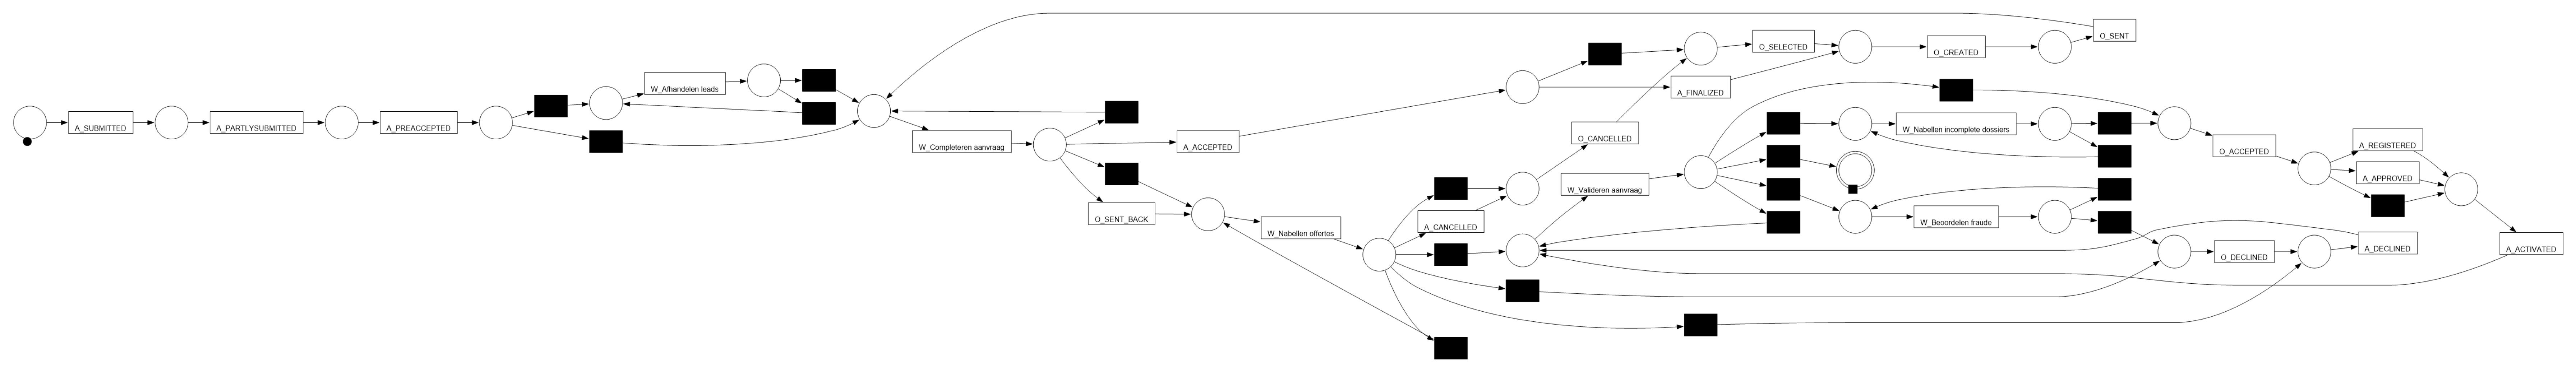
\includegraphics[width=\textwidth]{multi_obj/case_studies/BPI12/discovery_output/BPI12_best_petri_net.jpg}
\vspace{0.5em}

{\small Rete originale --- \texttt{A\_CANCELLED} ha una sola posizione}
\end{frame}

\begin{frame}{Rete di Petri --- DOPO}
\centering
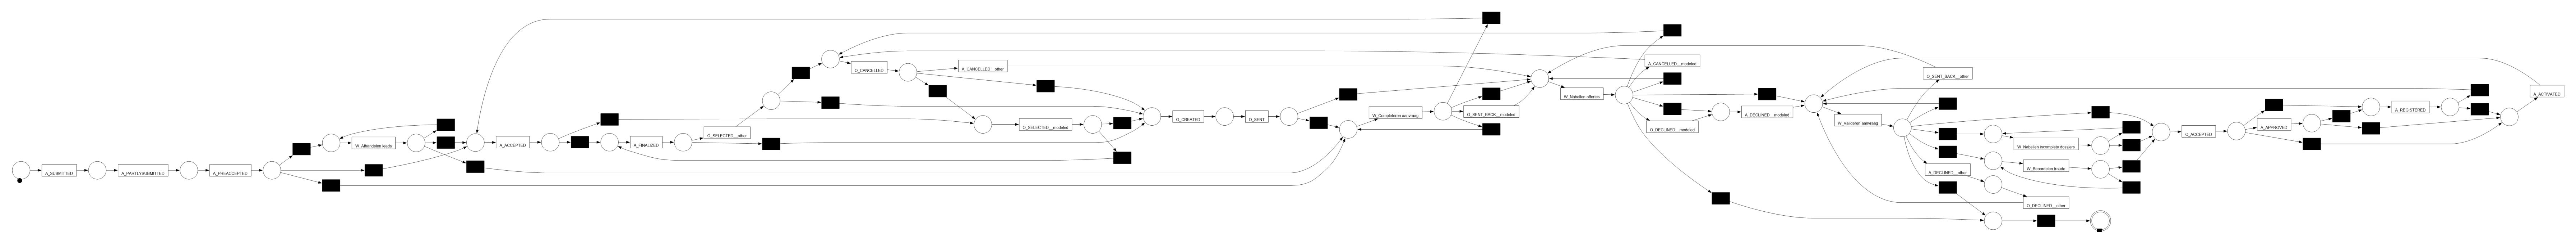
\includegraphics[width=\textwidth]{multi_obj/case_studies/BPI12_relabeled/discovery_output/log_BPI12_relabeled_best_petri_net.jpg}
\vspace{0.5em}

{\small Log rinominato (5 attivit\`a) + tuning Optuna --- ogni attivit\`a ambigua ora ha 2 transizioni distinte}
\end{frame}


\begin{frame}{La soluzione: rinominare nel log}
\begin{itemize}
\item Rinominare le occorrenze ambigue \textbf{prima} di Split Miner $\to$ l'algoritmo costruisce la rete da capo, in modo consistente
\item Criterio: predecessore reale gi\`a modellato $\to$ \texttt{\_\_modeled}; tutto il resto $\to$ \texttt{\_\_other}
\end{itemize}
\begin{center}
\scriptsize
\begin{tabular}{lll}
\toprule
\textbf{Attivit\`a} & \textbf{\_\_modeled} & \textbf{\_\_other (mancante)} \\
\midrule
A\_CANCELLED & W\_Nabellen offertes & O\_CANCELLED (46.8\%) \\
O\_SENT\_BACK & W\_Completeren aanvraag & W\_Nabellen offertes (77.7\%) \\
O\_DECLINED & W\_Nabellen offertes & A\_DECLINED (47.8\%) \\
O\_SELECTED & A\_ACCEPTED, O\_CANCELLED & A\_FINALIZED (29.9\%) \\
A\_DECLINED & W\_Nabellen off., O\_DECLINED & W\_Valideren aanvraag (14.1\%) \\
\bottomrule
\end{tabular}
\end{center}
\end{frame}

\begin{frame}{Risultati, passo per passo}
\centering
\scriptsize
\begin{tabular}{lccc}
\toprule
\textbf{Versione} & \textbf{Ev./traccia} & \textbf{\% esito +} & \textbf{A\_CANCELLED} \\
\midrule
\rowcolor{accentsoft} Reale & 24.3--24.6 & 48.3\% & 0.350 \\
1. Prob. fisse & \warncell{21.38} & \warncell{30.2\%} & \badcell{0.000} \\
2. Alberi, prima dei fix & \badcell{44.36} & 48.7\% & \badcell{5--7$\times$} \\
3. + 3 fix simulatore & \good{22.20} & 52.4\% & \badcell{0.000} \\
4. + patch manuale & 23.45 & 55.5\% & 0.195 \\
7. Rinomina, A\_CANCELLED & 23.04 & \dashcell & \good{0.347} \\
8. Rinomina, 5 attiv. & 21.09 & 46.4\% & \good{0.353} \\
\rowcolor{accentsoft} 9. Rinomina, 5 attiv., Optuna & \good{24.33} & 56.4\% & \good{0.345} \\
\bottomrule
\end{tabular}
\vspace{1em}

{\small Tabella completa (9 versioni + durata) nel report esteso}
\end{frame}

\begin{frame}{Durata delle tracce, passo per passo}
\centering
\small
\begin{tabular}{lccc}
\toprule
\textbf{Versione} & \textbf{Dur. media} & \textbf{Dur. mediana} & \textbf{Dur. massima} \\
\midrule
\rowcolor{accentsoft} Reale (BPI12) & 18.63 gg & 15.10 gg & 91.4 gg \\
1. Prob. fisse (depth=0) & 16.45 gg & 13.27 gg & 107.2 gg \\
4. + patch manuale (1 arco) & 21.17 gg & 15.12 gg & \warncell{335.7 gg} \\
7. Rinomina, solo A\_CANCELLED ($\varepsilon$/$\eta$ fissi) & 16.67 gg & 12.96 gg & 156.7 gg \\
8. Rinomina, 5 attivit\`a ($\varepsilon$/$\eta$ fissi) & 17.05 gg & 12.00 gg & 146.1 gg \\
\rowcolor{accentsoft} 9. Rinomina, 5 attivit\`a, Optuna & 20.94 gg & \good{17.13 gg} & \warncell{287.5 gg} \\
\bottomrule
\end{tabular}
\vspace{0.8em}

{\small Passi 2, 3, 5, 6: durata non misurata a quel punto dell'indagine.\\
La mediana del passo 9 \`e la pi\`u vicina al reale; la coda (massimo) resta un limite aperto ovunque si usi l'instradamento condizionato.}
\end{frame}

\begin{frame}{Confronto per attivit\`a --- ultimo passo (Optuna) (1/2)}
\centering
\scriptsize
\begin{tabular}{lcccc}
\toprule
\textbf{Attivit\`a} & \textbf{Reale (media/max)} & \textbf{Sim (media/max)} & \textbf{Rapporto} \\
\midrule
W\_Valideren aanvraag & 1.648 / 28 & 2.037 / 13 & \warncell{1.24} \\
O\_ACCEPTED & 0.479 / 1 & 0.592 / 3 & \warncell{1.24} \\
W\_Nabellen offertes & 4.587 / 33 & 5.103 / 39 & 1.11 \\
A\_ACTIVATED & 0.479 / 1 & 0.504 / 3 & 1.05 \\
W\_Nabellen incomplete dossiers & 2.326 / 60 & 2.435 / 52 & 1.05 \\
A\_FINALIZED & 1.000 / 1 & 1.004 / 3 & \good{1.00} \\
A\_PARTLYSUBMITTED & 1.000 / 1 & 1.000 / 1 & \good{1.00} \\
A\_PREACCEPTED & 1.000 / 1 & 1.000 / 1 & \good{1.00} \\
A\_SUBMITTED & 1.000 / 1 & 1.000 / 1 & \good{1.00} \\
A\_ACCEPTED & 1.000 / 1 & 0.997 / 2 & \good{1.00} \\
W\_Completeren aanvraag & 2.376 / 25 & 2.351 / 23 & \good{0.99} \\
A\_CANCELLED & 0.350 / 1 & 0.345 / 5 & \good{0.98} \\
\bottomrule
\end{tabular}
\vspace{0.8em}

{\small ``Media'' = occorrenze medie per traccia; ``max'' = il pi\`u alto numero di ripetizioni osservato in una singola traccia (reale 4685 tracce, simulato 5232 tracce). 23 attivit\`a totali, ordinate per rapporto decrescente -- segue (2/2).}
\end{frame}

\begin{frame}{Confronto per attivit\`a --- ultimo passo (Optuna) (2/2)}
\centering
\scriptsize
\begin{tabular}{lcccc}
\toprule
\textbf{Attivit\`a} & \textbf{Reale (media/max)} & \textbf{Sim (media/max)} & \textbf{Rapporto} \\
\midrule
O\_CREATED & 1.396 / 7 & 1.355 / 5 & \good{0.97} \\
O\_SENT & 1.396 / 7 & 1.355 / 5 & \good{0.97} \\
A\_DECLINED & 0.171 / 1 & 0.154 / 3 & 0.90 \\
O\_SELECTED & 1.396 / 7 & 1.170 / 4 & 0.84 \\
W\_Afhandelen leads & 0.344 / 9 & 0.286 / 7 & 0.83 \\
O\_CANCELLED & 0.746 / 6 & 0.604 / 5 & 0.81 \\
A\_APPROVED & 0.479 / 1 & 0.309 / 3 & \warncell{0.64} \\
O\_DECLINED & 0.171 / 1 & 0.105 / 3 & \warncell{0.62} \\
O\_SENT\_BACK & 0.715 / 3 & 0.382 / 3 & \warncell{0.53} \\
A\_REGISTERED & 0.479 / 1 & 0.239 / 3 & \warncell{0.50} \\
W\_Beoordelen fraude & 0.011 / 4 & 0.003 / 3 & \warncell{0.30} \\
\bottomrule
\end{tabular}
\vspace{0.8em}

{\small A\_APPROVED, A\_REGISTERED, W\_Beoordelen fraude non facevano parte delle 5 attivit\`a rinominate: la loro deviazione riflette limiti residui del modello di instradamento, non il problema dei duplicate task.}
\end{frame}

\begin{frame}{Limiti residui}
\begin{itemize}
\item \textbf{O\_SENT\_BACK}: migliorato (0.13$\to$0.38 su 0.72 reale) ma ancora sottostimato
\item O\_DECLINED, O\_SELECTED, O\_CANCELLED: sottostimati (rapporto 0.6--0.8)
\item Coda delle tracce lunghe: durata massima 2--3$\times$ il reale, anche nella versione migliore
\item \% esito positivo: 56.4\% contro 48.3\% reale --- Optuna ottimizza fitness/precisione globali, non questa metrica
\item Le altre attivit\`a ``diffuse'' non toccate
\end{itemize}
\end{frame}

\begin{frame}{Raccomandazione}
\begin{block}{}
Documentare il percorso completo --- \`e gi\`a un contributo metodologico solido: causa radice identificata, verifica quantitativa, tentativi scartati con motivazione, soluzione funzionante.
\end{block}
\vspace{1em}
Usare la versione Optuna (passo 9) come dataset di riferimento, elencando i limiti residui come lavoro futuro esplicito.
\end{frame}

\begin{frame}{Appendice: gli alberi decisionali dentro ProSiT}
\centering
\scriptsize
\begin{tabular}{lllp{4.7cm}}
\toprule
\textbf{Albero} & \textbf{Uno per} & \textbf{Tipo} & \textbf{Cosa predice} \\
\midrule
Instradamento (control-flow) & transizione della rete & classificazione & scatta adesso, s\`i/no? (peso nel sorteggio tra le transizioni abilitate) \\
Tempo di esecuzione & attivit\`a & regressione & minuti di lavoro effettivo (al netto del calendario risorsa) \\
Tempo di attesa & risorsa & regressione & minuti di attesa prima dell'inizio \\
Tempo tra arrivi & globale & regressione & minuti tra un nuovo caso e il successivo \\
\bottomrule
\end{tabular}
\vspace{0.8em}

{\small \texttt{max\_depth\_tree} (parametro CLI usato in tutta l'indagine, tipicamente 2--3) controlla tutti e quattro: se $<1$ si torna alla modalit\`a ``flat'' (nessun albero, solo frequenza empirica); altrimenti \`e la profondit\`a massima esplorata.}
\end{frame}

\begin{frame}{Appendice: parametri e selezione della profondit\`a}
\begin{itemize}
\item Modello: \texttt{sklearn.tree.DecisionTreeClassifier} (instradamento) / \texttt{DecisionTreeRegressor} (tempi)
\item Regolarizzazione, \textbf{identica sui 4 alberi}: \texttt{min\_samples\_leaf=100}, \texttt{min\_samples\_split=200} 
\item \texttt{random\_state=72} per riproducibilit\`a
\item Profondit\`a scelta con \texttt{GridSearchCV(cv=3)} su \texttt{max\_depth} $\in\{1,\dots,\texttt{max\_depth\_tree}\}$, criterio di default (accuracy / R\textsuperscript{2}); se il fit fallisce (pochi campioni) fallback ad un albero fisso di profondit\`a 1--2
\end{itemize}
\end{frame}

\begin{frame}{Appendice: encoding delle feature in input}
\begin{itemize}
\item \textbf{Storico di caso}: un contatore intero per ciascuna etichetta della rete = quante volte quell'attivit\`a \`e gi\`a avvenuta in \emph{questa} traccia finora --- non one-hot, valore intero crescente, aggiornato ad ogni evento
\item \textbf{Attributi di traccia/evento}: rilevati automaticamente come ogni colonna del log oltre a quelle standard XES (case id, attivit\`a, timestamp, risorsa, ruolo). Se il valore \`e testuale $\to$ one-hot (\texttt{attributo = valore}); se numerico $\to$ colonna grezza
\item Solo per il \textbf{tempo di esecuzione}: risorsa che esegue, one-hot (\texttt{resource = nome})
\item Solo per il \textbf{tempo di attesa}: \texttt{workload} = numero di altri eventi che la stessa risorsa stava gestendo nell'istante in cui la transizione si \`e abilitata
\item Tutto tabellare: nessuna feature testuale libera, nessun embedding
\end{itemize}
\end{frame}


\begin{frame}{Riprodurre l'indagine}
\begin{itemize}
\item \texttt{discovery/analyze\_duplicate\_task\_candidates.py} --- screening
\item \texttt{discovery/repair\_pruned\_concurrent\_edges.py} --- riferimento storico
\item \texttt{discovery/relabel\_and\_test\_duplicate\_task.py} --- lo strumento che ha funzionato
\item \texttt{discovery/petri\_net\_discovery.py} --- tuning Optuna completo
\end{itemize}
\vspace{1em}
\centering\Large\color{accent} Grazie
\end{frame}

\end{document}
